%        File: hw2.tex
%     Created: Sun Oct 2 05:00 PM 2013 E
% Last Change: Sun Oct 2 05:00 PM 2013 E
%
\documentclass[a4paper]{report}

\title{HW 3}
\author{Delos Chang}
\date{}

\usepackage{amsmath, amsthm, amssymb, fancyhdr, tikz}
\usetikzlibrary{arrows}
\newcommand{\justif}[2]{&{#1}&\text{#2}}

\pagestyle{fancy}
\rhead{HW 3:  Delos Chang (help from Prof.)}
\begin{document}
  \begin{enumerate}
    %&=& &=& &=& &=& &=& &=& &=& &=& &=& &=& &=& &=& &=& &=& &=& =
    % Question 1 
    %&=& &=& &=& &=& &=& &=& &=& &=& &=& &=& &=& &=& &=& &=& &=& =
    \item
      **In a tree, for any two nodes $a$ and $b$, a unique path exists from $a$ to $b$.

      - Run BFS from any arbitrary node $u$ in the graph $T=(V,E)$. Mark the node $v$ with the highest discovery time in the BFS, 
      i.e. the node that is discovered last. $v$ must be a leaf node. 

      - Run BFS starting from node $v$. Mark the node $v_2$ with the highest discovery time in the BFS i.e. the node that is discovered last. 
      $\delta(v,v_2)$ is the diameter of the tree $T$. 




    %&=& &=& &=& &=& &=& &=& &=& &=& &=& &=& &=& &=& &=& &=& &=& =
    % Question 2 
    %&=& &=& &=& &=& &=& &=& &=& &=& &=& &=& &=& &=& &=& &=& &=& =
    \par
    \bigskip

    \item
      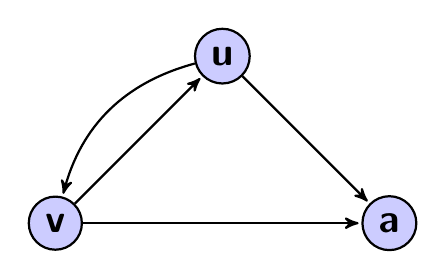
\begin{tikzpicture}[->,>=stealth',shorten >=1pt,auto,node distance=3cm,
        thick,main node/.style={circle,fill=blue!20,draw,font=\sffamily\Large\bfseries}]

        \node[main node] (1) {u};
        \node[main node] (2) [below left of=1] {v};
        \node[main node] (4) [below right of=1] {a};

        \path[every node/.style={font=\sffamily\small}]
        (1) edge node [left] {} (4)
        edge [bend right] node[left] {} (2)
        (2) edge node [right] {} (1)
        edge node {} (4);
      \end{tikzpicture}

      When DFS is run on the above counterexample where $d[u] < d[v]$ but $v$ is not a descendant of $u$ in the
      depth-first forest produced.

    %&=& &=& &=& &=& &=& &=& &=& &=& &=& &=& &=& &=& &=& &=& &=& =
    % Question 3 
    %&=& &=& &=& &=& &=& &=& &=& &=& &=& &=& &=& &=& &=& &=& &=& =
    \par
    \bigskip

    Same as $2$ but start DFS from $v$.

    %&=& &=& &=& &=& &=& &=& &=& &=& &=& &=& &=& &=& &=& &=& &=& =
    % Question 4 
    %&=& &=& &=& &=& &=& &=& &=& &=& &=& &=& &=& &=& &=& &=& &=& =
    \par
    \bigskip

    %&=& &=& &=& &=& &=& &=& &=& &=& &=& &=& &=& &=& &=& &=& &=& =
    % Question 4 
    %&=& &=& &=& &=& &=& &=& &=& &=& &=& &=& &=& &=& &=& &=& &=& =
    \par
    \bigskip






  \end{enumerate}
\end{document}


